\chapter{Catalyse organométallique~: étapes élémentaires et cycles}\label{ch:b2:catalytic-cycles}

Quelques milligrammes d'un sel de palladium peuvent unir deux cycles \omterm{def:b2:huckel:aromatic}{aromatiques} dans un ballon
contenant des kilogrammes de réactifs~: le même atome métallique fait le travail des milliers de
fois, en revenant à son état de départ après chaque passage. La manière dont il y parvient est
décrite par un \omterm{def:b2:catalytic-cycles:cycle}{cycle catalytique}, une suite fermée de quelques étapes élémentaires.
Il n'existe que peu de types d'étapes, et chacune modifie d'une façon fixée le degré d'oxydation, le
nombre d'électrons et le nombre de ligands du métal. Grâce au
décompte d'électrons du \cref{ch:b2:coordination-complexes}, on peut lire un cycle, le
vérifier, et parfois le prévoir.

\begin{recall}
\Cref{ch:b2:coordination-complexes}~: degré d'oxydation, $d^n$, \omterm{def:b2:coordination-complexes:electron-count}{nombre d'électrons de valence},
\omterm{def:b2:coordination-complexes:electron-count}{règle des 18 électrons}, \omterm{def:b2:coordination-complexes:hapticity}{hapticité}. \Cref{ch:b2:ligand-field}~: ligands $\pi$-accepteurs et
\omterm{def:b2:ligand-field:pi-ligands}{rétrodonation}. Le volume de première année~: catalyseur, catalyse homogène, acte élémentaire,
étape cinétiquement déterminante, composé organométallique, nombre d'oxydation.
\end{recall}

\begin{omfigure}
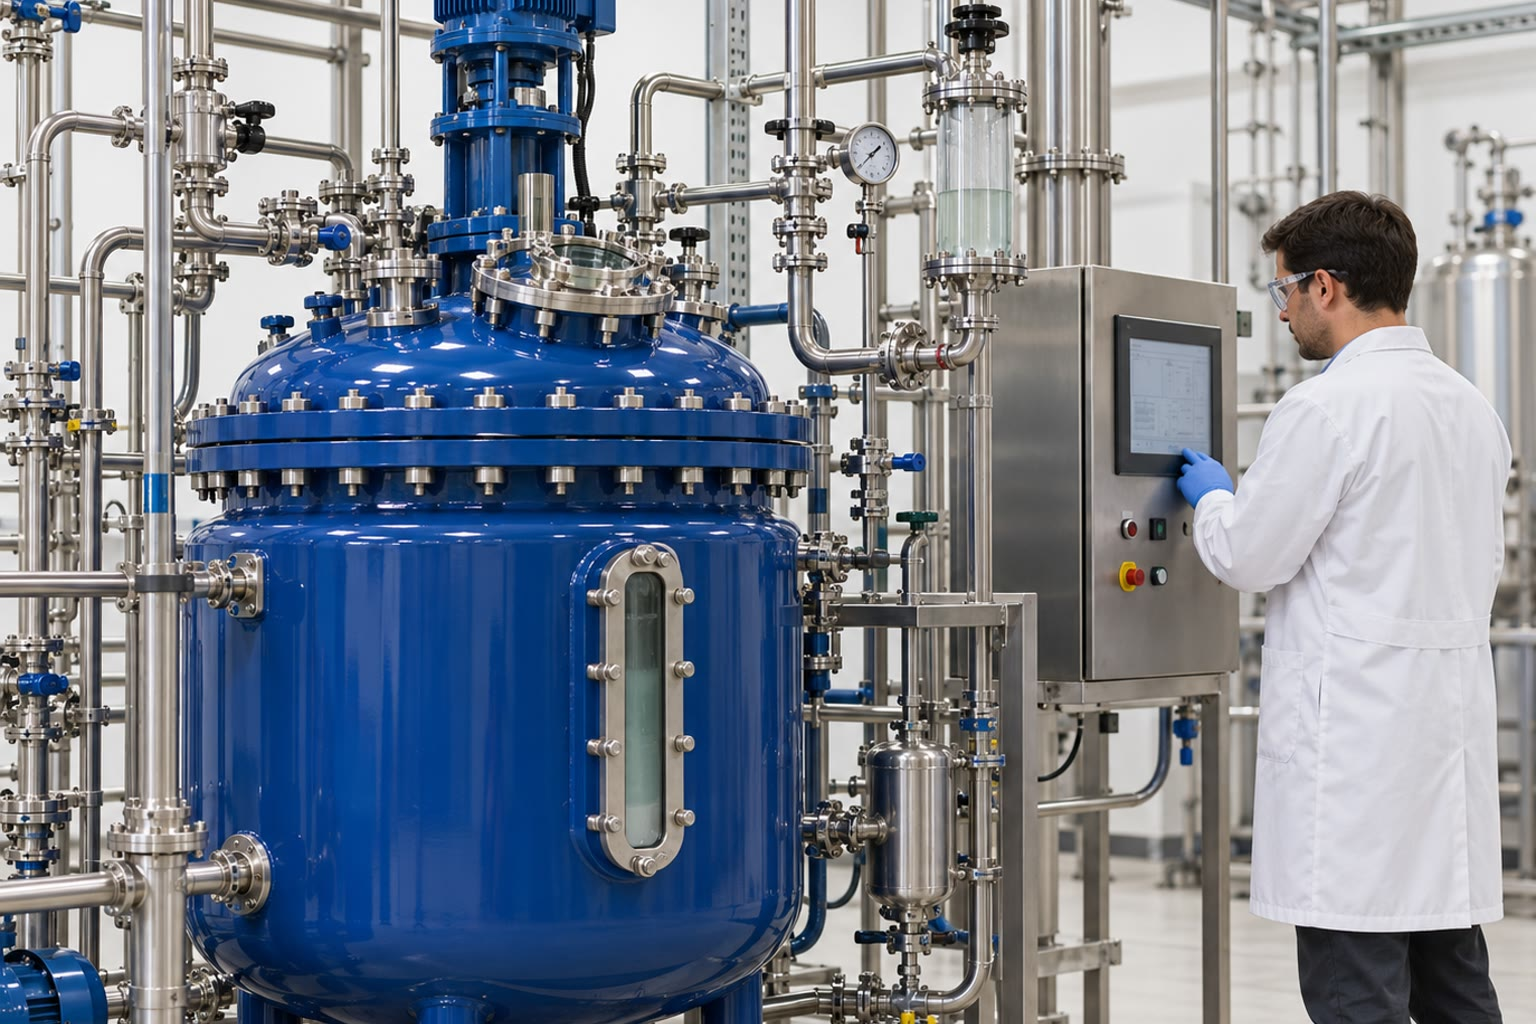
\includegraphics[width=0.62\linewidth]{images/book3/ai/b2-20-pilot-plant.jpg}

{\small Une installation pilote de chimie des procédés~: un réacteur en acier émaillé, où un
couplage catalysé est extrapolé à partir du ballon avant la production.}
\end{omfigure}

\section{Le langage des complexes organométalliques}

Les complexes organométalliques se décomptent comme dans la \cref{met:b2:coordination-complexes:electron-count},
avec quelques ligands supplémentaires~: un hydrure \ce{H-} et un anion alkyle ou aryle \ce{R-} apportent chacun deux
électrons et comptent pour $-1$ dans le degré d'oxydation~; \ce{CO}, les phosphines \ce{PR3} et
les $\eta^2$-alcènes apportent deux électrons et comptent pour 0~; un halogénure \ce{X-} en apporte deux et compte
pour $-1$.

\begin{definition}[Complexes insaturés]\label{def:b2:catalytic-cycles:unsaturated}
Un \emph{complexe coordinativement insaturé}\index{complexe coordinativement insature@complexe coordinativement insaturé}
possède moins de 18 électrons de valence (souvent 16) et peut fixer un autre ligand~: il possède un
\emph{site vacant}\index{site vacant}, une position de sa \omterm{def:b2:coordination-complexes:coordination-sphere}{sphère de coordination} libre pour
recevoir un donneur de deux électrons.
\end{definition}

Les complexes $d^8$ plans carrés du rhodium(I), de l'iridium(I), du palladium(II) et du
platine(II) sont des complexes à 16 électrons~; les bisphosphines du palladium(0) \ce{PdL2} en ont 14.
De tels complexes sont les espèces actives de la plupart des \omterm{def:b2:catalytic-cycles:cycle}{cycles catalytiques}.

\begin{method}[Décompter un complexe organométallique]\label{met:b2:catalytic-cycles:count-organometallic}
\begin{enumerate}
  \item Recenser les ligands~: anioniques (\ce{H-}, \ce{R-}, \ce{X-}, \ce{C5H5-}) et neutres
        (\ce{CO}, \ce{PR3}, alcènes, solvant).
  \item Degré d'oxydation = charge du complexe $-$ somme des charges des ligands anioniques.
  \item $n = g -$ degré d'oxydation~; décompte = $n + 2 \times$(nombre de donneurs de deux électrons)
        $+$ 6 par $\eta^5$-\ce{C5H5-}.
  \item Coordinence = nombre de positions de ligand occupées.
\end{enumerate}
\end{method}

\section{Échange de ligand, addition oxydante, élimination réductrice}

\begin{definition}[Échange de ligand]\label{def:b2:catalytic-cycles:ligand-exchange}
Un \emph{échange de ligand}\index{echange de ligand@échange de ligand} est une étape élémentaire au cours de laquelle un ligand de
la \omterm{def:b2:coordination-complexes:coordination-sphere}{sphère de coordination} est remplacé par un autre~; il ne modifie ni le degré d'oxydation
ni, globalement, le nombre d'électrons. Ses mécanismes sont étudiés dans le volume de troisième année.
\end{definition}

\begin{definition}[Addition oxydante et élimination réductrice]\label{def:b2:catalytic-cycles:oxidative-addition}
Lors d'une \emph{addition oxydante}\index{addition oxydante}, une molécule A--B s'additionne sur un
centre métallique en rompant sa liaison A--B et en formant des liaisons M--A et M--B. Une
\emph{élimination réductrice}\index{elimination reductrice@élimination réductrice} est l'étape inverse~: deux
ligands A et B, en cis l'un de l'autre, s'unissent en A--B et quittent le métal.
\end{definition}

\begin{proposition}[Décompte d'une addition oxydante]\label{prop:b2:catalytic-cycles:oa}
Une \omterm{def:b2:catalytic-cycles:oxidative-addition}{addition oxydante} augmente de 2 le degré d'oxydation du métal, son \omterm{def:b2:coordination-complexes:electron-count}{nombre d'électrons
de valence} et sa coordinence~; une \omterm{def:b2:catalytic-cycles:oxidative-addition}{élimination réductrice} les diminue chacun de 2.
\end{proposition}

\begin{proof}
A et B sont comptés comme des anions (\ce{H-}, \ce{R-}, \ce{X-}) une fois liés~: deux nouveaux ligands
anioniques augmentent le degré d'oxydation de 2 et diminuent $n$ de 2~; ils apportent deux doublets, $+4$
électrons~; le décompte varie de $-2 + 4 = +2$. Deux positions sont nouvellement occupées. L'étape
inverse inverse chacune de ces variations.
\end{proof}

\begin{example}[Le complexe de Vaska]\label{ex:b2:catalytic-cycles:vaska}
\ce{[IrCl(CO)(PPh3)2]}, plan carré~: iridium(I), $d^8$, 16 électrons, tétracoordiné.
Il additionne le dihydrogène~: \ce{[IrH2Cl(CO)(PPh3)2]}, iridium(III), $d^6$, 18 électrons, octaédrique,
les deux hydrures étant en cis.
\end{example}

\section{Insertion, élimination, transmétallation}

\begin{definition}[Insertion et $\beta$-élimination d'hydrure]\label{def:b2:catalytic-cycles:insertion}
Lors d'une \emph{insertion migratoire}\index{insertion migratoire}, un ligand insaturé
(alcène, \ce{CO}) lié au métal s'insère dans une liaison M--H ou M--C en cis~: \ce{M-H} et un
alcène donnent un alkyle \ce{M-CH2-CH2-H}~; \ce{M-R} et \ce{CO} donnent un acyle \ce{M-C(=O)R}.
Une \emph{$\beta$-élimination d'hydrure}\index{beta-elimination d'hydrure@$\beta$-élimination d'hydrure}
est l'inverse d'une insertion d'alcène~: un hydrogène porté par le carbone en $\beta$ du
métal passe sur le métal, ce qui libère un alcène.
\end{definition}

\begin{proposition}[Décompte d'une insertion]\label{prop:b2:catalytic-cycles:insertion}
Une \omterm{def:b2:catalytic-cycles:insertion}{insertion migratoire} conserve le degré d'oxydation et diminue de 2 le nombre d'électrons
(une position de ligand est libérée)~; une $\beta$-élimination d'hydrure l'augmente de 2.
\end{proposition}

\begin{proof}
Avant~: \ce{H-} (ou \ce{R-}, anionique) et l'alcène (neutre), deux ligands, quatre électrons.
Après~: un alkyle (anionique), deux électrons. La charge anionique est inchangée~: même
degré d'oxydation~; deux électrons et une position sont perdus.
\end{proof}

\begin{proposition}[Conditions de la $\beta$-élimination d'hydrure]\label{prop:b2:catalytic-cycles:beta-h}
Un alkylmétal ne subit de $\beta$-élimination d'hydrure que si l'alkyle porte un hydrogène sur
son carbone $\beta$ et si le métal possède un \omterm{def:b2:catalytic-cycles:unsaturated}{site vacant} en cis de l'alkyle.
\end{proposition}

\begin{proof}[Argument]
L'étape passe par un arrangement à quatre centres M--C$_\alpha$--C$_\beta$--H dans lequel
l'hydrogène atteint le métal~: elle exige cet hydrogène, et une position vide voisine de l'alkyle
pour le recevoir. Les groupes méthyle, benzyle, néopentyle et aryle, qui n'ont pas d'hydrogène $\beta$
capable d'atteindre le métal, y sont stables.
\end{proof}

\begin{definition}[Transmétallation]\label{def:b2:catalytic-cycles:transmetalation}
Une \emph{transmétallation}\index{transmetallation@transmétallation} transfère un groupe organique d'un métal
(ou d'un métalloïde~: bore, zinc, étain) à un autre, en général en échange d'un halogénure.
\end{definition}

\begin{omfigure}
\begin{tikzpicture}[font=\small, >={Stealth}]
  \tikzset{omstepar/.style={->, thick}}
  \foreach \y/\l/\r/\top/\bot/\rev in {
      0/{$\mathrm{L}_n\mathrm{M}$}/{$\mathrm{L}_n\mathrm{M(A)(B)}$}/{+ A--B}/{addition oxydante}/{élimination réductrice},
      -1.5/{$\mathrm{L}_n\mathrm{M(H)(CH_2{=}CH_2)}$}/{$\mathrm{L}_n\mathrm{M{-}CH_2CH_3}$}/{}/{insertion migratoire}/{$\beta$-élimination d'hydrure},
      -3.0/{$\mathrm{L}_n\mathrm{M(X)(R)}$}/{$\mathrm{L}_n\mathrm{M(R)(R')}$}/{+ R$'$--[B], $-$ X--[B]}/{transmétallation}/{},
      -4.5/{$\mathrm{L}_n\mathrm{M(X)}$}/{$\mathrm{L}_n\mathrm{M(X)(L')}$}/{+ L$'$}/{échange ou fixation de ligand}/{}} {
    \node[cyclenode, anchor=east] (l) at (0,\y) {\l};
    \node[cyclenode, anchor=west] (r) at (5.2,\y) {\r};
    \draw[omstepar] ($(l.east)+(0.1,0.08)$) -- ($(r.west)+(-0.1,0.08)$) node[midway, above, font=\scriptsize] {\top};
    \node[font=\scriptsize, anchor=north] at (2.6,\y-0.02) {\bot};
    \node[font=\scriptsize, black!55, anchor=west] at (5.2,\y-0.5) {\rev};
  }
\end{tikzpicture}

{\small Les étapes élémentaires de la catalyse organométallique. \omterm{def:b2:catalytic-cycles:oxidative-addition}{Addition oxydante}~: degré
d'oxydation, décompte et coordinence $+2$~; \omterm{def:b2:catalytic-cycles:oxidative-addition}{élimination réductrice}~: $-2$. \omterm{def:b2:catalytic-cycles:insertion}{Insertion
migratoire}~: décompte $-2$, degré d'oxydation inchangé~; $\beta$-élimination d'hydrure~:
l'inverse. \omterm{def:b2:catalytic-cycles:transmetalation}{Transmétallation}~: un groupe organique passe au métal depuis le bore, le zinc ou l'étain.}
\end{omfigure}

\section{Lire un cycle catalytique}

\begin{definition}[Cycle catalytique]\label{def:b2:catalytic-cycles:cycle}
Un \emph{cycle catalytique}\index{cycle catalytique} est une suite fermée d'étapes élémentaires
qui consomme les réactifs, libère les produits et régénère son premier complexe. Le
composé ajouté au milieu réactionnel, qui se transforme en premier complexe du cycle, est le
\emph{précatalyseur}\index{precatalyseur@précatalyseur}. Le \emph{nombre de cycles}\index{nombre de cycles}
(TON) est la quantité de produit formée par quantité de catalyseur~; la \emph{fréquence de
cycles}\index{frequence de cycles@fréquence de cycles} (TOF) est le nombre de cycles par unité de temps.
\end{definition}

\begin{proposition}[L'équation globale]\label{prop:b2:catalytic-cycles:cycle-sum}
La somme des étapes d'un \omterm{def:b2:catalytic-cycles:cycle}{cycle catalytique} est l'équation de la réaction catalysée~:
chaque complexe métallique apparaît une fois comme produit et une fois comme réactif, et se simplifie.
\end{proposition}

\begin{proof}
Le cycle étant fermé, chaque intermédiaire est formé par une étape et consommé par la suivante~;
en additionnant les étapes, ces espèces apparaissent des deux côtés et se simplifient. Il reste les
espèces qui entrent de l'extérieur (réactifs) et qui sortent (produits).
\end{proof}

\begin{method}[Lire un cycle]\label{met:b2:catalytic-cycles:read-cycle}
\begin{enumerate}
  \item Pour chaque complexe, calculer le degré d'oxydation, le nombre d'électrons et la
        coordinence.
  \item Nommer chaque étape d'après les variations ($+2/+2/+2$~: \omterm{def:b2:catalytic-cycles:oxidative-addition}{addition oxydante}~; décompte $-2$ à
        degré d'oxydation constant~: insertion~; et ainsi de suite).
  \item Vérifier qu'aucun complexe ne dépasse 18 électrons et qu'une étape qui exige un \omterm{def:b2:catalytic-cycles:unsaturated}{site vacant}
        part d'un complexe insaturé.
  \item Additionner les étapes~: la somme doit être l'équation globale.
\end{enumerate}
\end{method}

\begin{omfigure}
\begin{tikzpicture}[font=\small, >={Stealth}]
  \node[cyclenode] (n1) at (90:2.3) {\ce{[RhCl(PPh3)2]}\\ Rh(I), 14 e};
  \node[cyclenode] (n2) at (0:3.4) {\ce{[RhH2Cl(PPh3)2]}\\ Rh(III), 16 e};
  \node[cyclenode] (n3) at (270:2.3) {\ce{[RhH2Cl(PPh3)2(RCH=CH2)]}\\ Rh(III), 18 e};
  \node[cyclenode] (n4) at (180:3.4) {\ce{[RhH(CH2CH2R)Cl(PPh3)2]}\\ Rh(III), 16 e};
  \draw[cyclearc] (n1) to[bend left=20] node[cyclelabel, below left] {addition\\ oxydante} (n2);
  \draw[cyclearc] (n2) to[bend left=20] node[cyclelabel, left=12pt] {fixation\\ de l'alcène} (n3);
  \draw[cyclearc] (n3) to[bend left=20] node[cyclelabel, above right] {insertion\\ migratoire} (n4);
  \draw[cyclearc] (n4) to[bend left=20] node[cyclelabel, below right] {élimination\\ réductrice} (n1);
  \draw[cyclein] (4.6,2.3) node[right] {\ce{H2}} -- (2.6,1.75);
  \draw[cyclein] (4.6,-2.3) node[right] {alcène} -- (2.6,-1.75);
  \draw[cycleout] (-2.6,1.75) -- (-4.6,2.3) node[left] {alcane};
  \node[font=\scriptsize, align=center, black!60] at (0,-0.05) {précatalyseur\\ \ce{[RhCl(PPh3)3]}\\ qui perd une \ce{PPh3}};
\end{tikzpicture}

{\small L'hydrogénation d'un alcène par le catalyseur de Wilkinson, simplifiée (échanges de phosphine
et de solvant omis). Les quatre étapes ont pour somme $\ce{RCH=CH2 + H2 -> RCH2CH3}$~; les
complexes du rhodium se simplifient.}
\end{omfigure}

\begin{omfigure}
\begin{tikzpicture}[font=\small, >={Stealth}]
  \node[cyclenode] (s1) at (90:2.3) {\ce{PdL2}\\ Pd(0), 14 e};
  \node[cyclenode] (s2) at (0:3.4) {\ce{[ArPd(Br)L2]}\\ Pd(II), 16 e};
  \node[cyclenode] (s3) at (270:2.3) {$[\mathrm{ArPd(Ar')L_2}]$\\ Pd(II), 16 e};
  \draw[cyclearc] (s1) to[bend left=25] node[cyclelabel, below left] {addition\\ oxydante} (s2);
  \draw[cyclearc] (s2) to[bend left=25] node[cyclelabel, above left] {transmétallation} (s3);
  \draw[cyclearc] (s3) to[bend left=35] node[cyclelabel, right] {élimination\\ réductrice} (s1);
  \draw[cyclein] (4.8,2.2) node[right] {\ce{Ar-Br}} -- (2.6,1.6);
  \draw[cyclein] (5.4,-0.9) node[right, align=left] {$\mathrm{Ar'B(OH)_2}$\\ + base} -- (3.3,-1.2);
  \draw[cycleout] (2.3,-2.0) -- (4.4,-2.9) node[right] {\ce{Br-}, \ce{B(OH)3}};
  \draw[cycleout] (-1.75,-0.4) -- (-4.2,-0.4) node[left] {$\mathrm{Ar{-}Ar'}$};
\end{tikzpicture}

{\small Le couplage de Suzuki, simplifié. Le palladium(0) additionne le bromure d'aryle~; la base
transforme l'acide boronique en borate, qui transfère son groupe aryle au palladium~; les deux
aryles, en cis, sont éliminés sous forme de biaryle, ce qui régénère le palladium(0).}
\end{omfigure}

Dans la réaction de Heck, le complexe aryle--palladium formé par \omterm{def:b2:catalytic-cycles:oxidative-addition}{addition oxydante} fixe un
alcène au lieu d'un borate~; l'\omterm{def:b2:catalytic-cycles:insertion}{insertion migratoire} place l'aryle sur l'alcène, et une
$\beta$-élimination d'hydrure libère l'alcène substitué (en général l'isomère trans)
et un hydrure de palladium, auquel une base retire \ce{HBr} pour régénérer le palladium(0).

L'hydroformylation, addition de \ce{H2} et de \ce{CO} sur un alcène pour donner un aldéhyde,
fait intervenir des hydrures de cobalt ou de rhodium~: insertion de l'alcène, insertion de \ce{CO}
dans la liaison métal--alkyle, \omterm{def:b2:catalytic-cycles:oxidative-addition}{addition oxydante} de \ce{H2} et \omterm{def:b2:catalytic-cycles:oxidative-addition}{élimination réductrice} de
l'aldéhyde. Le sens de la première insertion décide du produit~: le métal sur le
carbone terminal donne l'aldéhyde linéaire, sur le carbone interne l'aldéhyde ramifié~; les phosphines
encombrées favorisent le produit linéaire.

\begin{history}[Les couplages croisés]
\begin{minipage}[t]{0.36\linewidth}
\vspace{0pt}
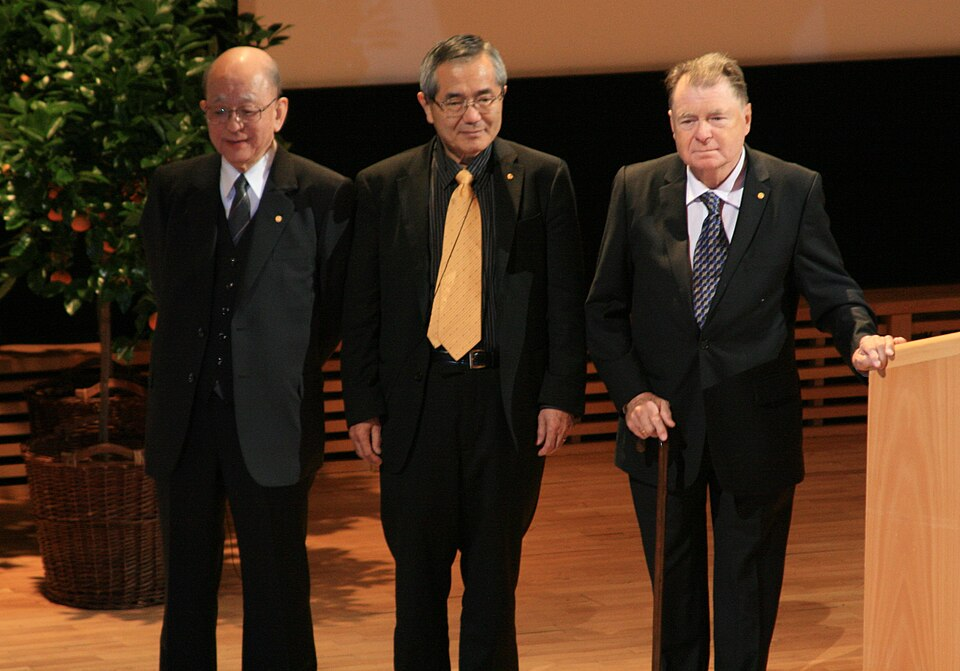
\includegraphics[width=\linewidth]{images/book3/nobel-2010.jpg}
\end{minipage}\hfill
\begin{minipage}[t]{0.6\linewidth}
\vspace{0pt}
Les couplages catalysés par le palladium des halogénures d'aryle et de vinyle avec les alcènes (Richard Heck, à partir de
1968), avec les organozinciques (Ei-ichi Negishi, 1977) et avec les composés organoborés
(Akira Suzuki, 1979) ont rendu routinière la jonction de deux squelettes carbonés~; ils comptent aujourd'hui parmi
les réactions les plus utilisées dans la fabrication des médicaments et des matériaux. Le prix Nobel de
chimie a été décerné aux trois chercheurs en 2010. (Photographie~: Suzuki, Negishi et Heck, de gauche
à droite, 2010~; BloodIce, CC BY-SA 4.0, Wikimedia Commons.)
\end{minipage}
\end{history}

\begin{proposition}[Nombre et fréquence de cycles]\label{prop:b2:catalytic-cycles:tof}
Si $n_P$ est la quantité de produit formée pendant une durée $t$ par une quantité $n_{\text{cat}}$ de catalyseur,
$\mathrm{TON} = n_P/n_{\text{cat}}$ et la fréquence moyenne de cycles vaut $\mathrm{TOF} =
\mathrm{TON}/t$.
\end{proposition}

\begin{proof}
Chaque tour du cycle forme une molécule de produit par atome métallique~; le nombre de tours accomplis
par chaque atome en moyenne vaut $n_P/n_{\text{cat}}$, et la vitesse de rotation est ce nombre par unité
de temps.
\end{proof}

\begin{safety}{\ghs[5mm]{GHS05}\,\ghs[5mm]{GHS07}\,\ghs[5mm]{GHS09}}
L'éthanoate de palladium(II) est corrosif pour les yeux et toxique pour les organismes aquatiques~;
la triphénylphosphine est nocive et sensibilisante. On les pèse sous hotte, et les
résidus de palladium sont collectés pour récupération, jamais jetés à l'évier.
% ledger: ghs:Pd-acetate, ghs:PPh3, ghs:phenylboronic-acid, ghs:4-bromotoluene
\end{safety}

\section{Exercices}

\begin{exercise}[$\star$]\label{exo:b2:catalytic-cycles:1}
Donner le degré d'oxydation, le $d^n$ et le nombre d'électrons du complexe de Vaska
\ce{[IrCl(CO)(PPh3)2]} avant et après l'addition de \ce{H2}.
\end{exercise}

\begin{exercise}[$\star$]\label{exo:b2:catalytic-cycles:2}
Nommer l'étape~: \ce{[PtCl2(CH3)2(PR3)2] -> [PtCl2(PR3)2] + C2H6}~; \ce{[Pd(Ph)Br(PR3)2] +
CH2=CH2 -> [Pd(CH2CH2Ph)Br(PR3)] + PR3}.
\end{exercise}

\begin{exercise}[$\star$]\label{exo:b2:catalytic-cycles:3}
Une réaction utilise \qty{0.020}{mmol} de catalyseur et donne \qty{15.0}{mmol} de produit en
\qty{3.0}{h}. Calculer le TON et la TOF moyenne.
\end{exercise}

\begin{exercise}[$\star$]\label{exo:b2:catalytic-cycles:4}
Additionner les trois étapes du cycle de Suzuki et vérifier que le palladium se simplifie.
\end{exercise}

\begin{exercise}[$\star\star$]\label{exo:b2:catalytic-cycles:5}
Lesquels de ces complexes alkylpalladium peuvent subir une $\beta$-élimination d'hydrure~:
\ce{Pd-CH3}, \ce{Pd-CH2CH3}, \ce{Pd-CH2C(CH3)3}, \ce{Pd-CH2Ph}, \ce{Pd-CH(CH3)2}~?
\end{exercise}

\begin{exercise}[$\star\star$]\label{exo:b2:catalytic-cycles:6}
Prévoir le produit de la réaction de Heck de l'iodobenzène avec le propénoate de méthyle, ainsi que sa
géométrie.
\end{exercise}

\begin{exercise}[$\star\star$]\label{exo:b2:catalytic-cycles:7}
Écrire les aldéhydes linéaire et ramifié formés par l'hydroformylation du propène, et
expliquer quelle insertion conduit à chacun.
\end{exercise}

\begin{exercise}[$\star\star$]\label{exo:b2:catalytic-cycles:8}
Pourquoi \ce{[RhCl(PPh3)3]} ne peut-il additionner \ce{H2} qu'après avoir perdu une phosphine, alors que
\ce{[RhCl(PPh3)2]} l'additionne immédiatement~?
\end{exercise}

\begin{exercise}[$\star\star$]\label{exo:b2:catalytic-cycles:9}
Dans le couplage de Suzuki, pourquoi faut-il une base, et que fait-elle à l'acide boronique~?
\end{exercise}

\begin{exercise}[$\star\star\star$]\label{exo:b2:catalytic-cycles:10}
Un cycle proposé pour l'hydrogénation d'un alcène sur un complexe $d^8$ \ce{ML3X} (16 e)
commence par la fixation de l'alcène, qui donne un complexe à 20 électrons, puis l'\omterm{def:b2:catalytic-cycles:oxidative-addition}{addition oxydante}
de \ce{H2}. Trouver l'erreur et corriger l'ordre.
\end{exercise}

\begin{exercise}[$\star\star\star$]\label{exo:b2:catalytic-cycles:11}
La quantité de produit d'une réaction catalysée croît selon $n_P(t) = n_{\max}(1 - \mathrm e^{-t/\tau})$
avec $n_{\max} = \qty{10.0}{mmol}$, $\tau = \qty{40}{min}$ et \qty{0.010}{mmol} de catalyseur
(données de l'exercice). Calculer la TOF initiale et le TON final.
\end{exercise}

\begin{exercise}[$\star\star\star$]\label{exo:b2:catalytic-cycles:12}
Proposer un couplage croisé pour préparer le 4-méthoxybiphényle, en choisissant l'halogénure et l'acide
boronique, et écrire le cycle.
\end{exercise}

\section{Problème~: lire le cycle de Suzuki}

\begin{problem}[{Problème du week-end --- le précatalyseur et le palladium(0) actif,
l'addition oxydante, la transmétallation et l'élimination réductrice d'un couplage de Suzuki, le
rendement et le nombre de cycles, et les réactions parasites}]
\label{pb:b2:catalytic-cycles:1}
Essai (données de l'exercice)~: \qty{10.0}{mmol} de 4-bromotoluène, \qty{12.0}{mmol}
d'acide phénylboronique, \qty{20}{mmol} de carbonate de potassium, \qty{0.050}{mmol} d'éthanoate de
palladium(II) et \qty{0.10}{mmol} de triphénylphosphine dans un mélange de toluène, d'éthanol et
d'eau, chauffé sous diazote~; produit isolé~: \qty{1.51}{g} de 4-méthylbiphényle. Masses
molaires (\unit{g/mol})~: 4-bromotoluène 171.04, acide phénylboronique 121.93, 4-méthylbiphényle
168.24, éthanoate de palladium(II) 224.51.
% ledger: aw:C, aw:H, aw:Br, aw:B, aw:O, aw:Pd

\medskip
\noindent\textbf{Partie I --- Le catalyseur.}
\begin{enumerate}
  \item Donner le degré d'oxydation et le $d^n$ du palladium dans l'éthanoate de palladium(II).
  \item Dans le ballon, il est réduit en \ce{Pd(PPh3)2}. Donner son degré d'oxydation, son $d^n$ et
        son nombre d'électrons.
  \item Pourquoi ce complexe est-il coordinativement insaturé~?
  \item Pourquoi conduit-on la réaction sous diazote~?
  \item Quel est le rôle de l'excès de triphénylphosphine~?
  \item L'éthanoate de palladium(II) est-il le catalyseur ou le \omterm{def:b2:catalytic-cycles:cycle}{précatalyseur}~?
\end{enumerate}

\medskip
\noindent\textbf{Partie II --- Les étapes.}
\begin{enumerate}[resume]
  \item Écrire l'\omterm{def:b2:catalytic-cycles:oxidative-addition}{addition oxydante} du 4-bromotoluène et faire le décompte du produit.
  \item Que fait le carbonate à l'acide phénylboronique~?
  \item Écrire la \omterm{def:b2:catalytic-cycles:transmetalation}{transmétallation}.
  \item Pourquoi les deux groupes aryle doivent-ils être en cis avant l'étape suivante~?
  \item Écrire l'\omterm{def:b2:catalytic-cycles:oxidative-addition}{élimination réductrice} et faire le décompte de l'espèce du palladium formée.
  \item Additionner les trois étapes.
\end{enumerate}

\medskip
\noindent\textbf{Partie III --- Rendement et \omterm{def:b2:catalytic-cycles:cycle}{nombre de cycles}.}
\begin{enumerate}[resume]
  \item Quel réactif est limitant~?
  \item Calculer la quantité de produit isolée.
  \item Calculer le rendement.
  \item Calculer la charge catalytique en \%~molaire par rapport au bromure.
  \item Calculer le \omterm{def:b2:catalytic-cycles:cycle}{nombre de cycles} du palladium.
  \item L'essai a duré \qty{4.0}{h}. Calculer la fréquence moyenne de cycles par heure.
\end{enumerate}

\medskip
\noindent\textbf{Partie IV --- Les réactions parasites.}
\begin{enumerate}[resume]
  \item On trouve un peu de biphényle \ce{Ph-Ph}. Proposer un mode de formation.
  \item Pourquoi aucune $\beta$-élimination d'hydrure n'est-elle possible ici~?
  \item Un chlorure d'aryle réagit bien plus lentement que le bromure. Quelle étape en pâtit~?
  \item Que devient le palladium à la fin de la réaction, et pourquoi le récupère-t-on~?
  \item Pourquoi utilise-t-on un léger excès d'acide boronique~?
  \item Donner le \omterm{def:b2:catalytic-cycles:cycle}{nombre de cycles} du palladium dans l'essai.
\end{enumerate}
\end{problem}
